\documentclass[tikz,border=4pt]{standalone}
\usepackage{pgfplots}
\pgfplotsset{compat=1.18}

\begin{document}
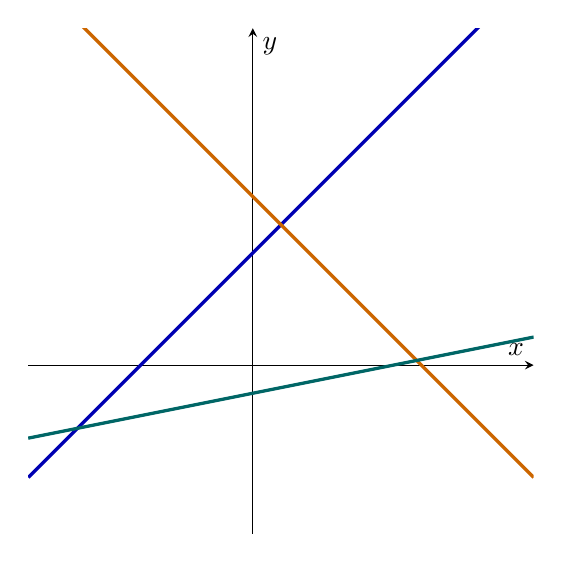
\begin{tikzpicture}
\begin{axis}[
    axis lines=center,
    xlabel={$x$},
    ylabel={$y$},
    xmin=-4, xmax=5,
    ymin=-3, ymax=6,
    xtick=\empty, ytick=\empty,
    width=8cm, height=8cm,
    clip=true
]

% Line 1: y = x + 2 (blue)
\addplot[domain=-4:5, samples=2, very thick, blue!70!black] {x + 2};

% Line 2: y = -x + 3 (orange)
\addplot[domain=-4:5, samples=2, very thick, orange!80!black] {-x + 3};

% Line 3: y = 0.2x - 0.5 (teal)
\addplot[domain=-4:5, samples=2, very thick, teal!80!black] {0.2*x - 0.5};

\end{axis}
\end{tikzpicture}
\end{document}
